\begin{bibunit}[plainnat]

\chapter{On Sampled Metrics for Item Recommendation}

Google Research \\

\textbf{Best research paper award}

\textbf{Reference:}~\url{http://walid.krichene.net/papers/KDD-sampled-metrics.pdf}

\textbf{Keywords:} ranking evaluation, metrics, sampling

\section*{Какую задачу решают авторы?}

Типичный протокол оценки качества рекомендательных систем выглядит следующим образом:
\begin{enumerate}
    \item Для отобранного множества пользователей $D$ ранжируем алгоритмом $A$ все множество кандидатов, состоящее из $n$ объектов
    \item Для каждого пользователя $\vecx$ вычисляем $R(A, \vecx)$ --- множество позиций релевантных объектов
    \item После чего для пользователя считаем метрику $M$, например, \texttt{ROC AUC} или \texttt{Precision@K}, \texttt{Recall@K}
\end{enumerate}

Итоговое значение метрики получается усредненеим метрик посчитанных по всем пользователям
\begin{equation*}
    \frac{1}{|D|}\sum\limits_{\vecx \in D} M(R(A, \vecx)) .
\end{equation*}

В ситуации когда $n$ велико часто прибегают к сэмплированию --- вместо того чтобы ранжировать все $n$ кандидатов, ранжируют случайную подвыборку из $m$ объектов ($ m \ll n $) вместе с релевантными для пользователя объектами. \\

Ожидается, что метрики посчитанные с сэмплированием позволяют упорядочить алгоритмы ранжирования по качеству так же как и метрики посчитанные без сэмплирования. 

Авторы статьи впервые тестируют это предположение и показывают что для большинства используемых метрик оно не верно, даже при многократном сэмплировании и усреднении результатов. \\

В статье предложены скорректированные варианты привычных метрик, которые позволяют при использовании сэмплирования сортировать алгоритмы по качеству также как если бы сэмплирования не было. 

\section*{Как решают?}

\textbf{Remark:} для простоты можно считать, что для каждого пользователя есть один релевантный объект. \\

Работу можно разбить на три части
\begin{enumerate}
    \item Экспериментальная часть, где проверяют предположение, что метрики с сэмплированием и без упорядочивают алгоритмы ранжирования одинаковым образом
    \item Теоретическая часть, посвященная скорректированным вариантам метрик
    \item Экспериментальная часть, где авторы показывают, что скорректированные варианты метрик работают
\end{enumerate}

\subsection*{Inconsistency of Sampled Metrics}

Ключевое определение данной работы

\ddef{Consistency}{
\label{def:consistenct}
Let the evaluation data $D$ be fixed. A metric $M$ is consistent under sampling if the relative order of any two recommenders $A$ and $B$ is preserved in expectation. That is, for all $A,B$,
\begin{align*}
    & \frac{1}{|D|} \sum\limits_{\vecx \in D} M(R(A,\vecx)) > \frac{1}{|D|} \sum\limits_{\vecx \in D} M(R(B,\vecx)) \\
    \Longleftrightarrow & \bE \left[ \frac{1}{|D|} \sum\limits_{\vecx \in D} M(\widetilde{R}(A,\vecx))  \right] > \bE \left[ \frac{1}{|D|} \sum\limits_{\vecx \in D} M(\widetilde{R}(B,\vecx))  \right]
\end{align*}
}

В рамках первой группы экспериментов (см. Рисунок~\ref{fig:example_vary_m}) показывают как меняются метрики для разных алгоритмов в зависимости от $m$ (число случайно отобранных объектов). \\

\begin{figure}[ht]
    \centering
    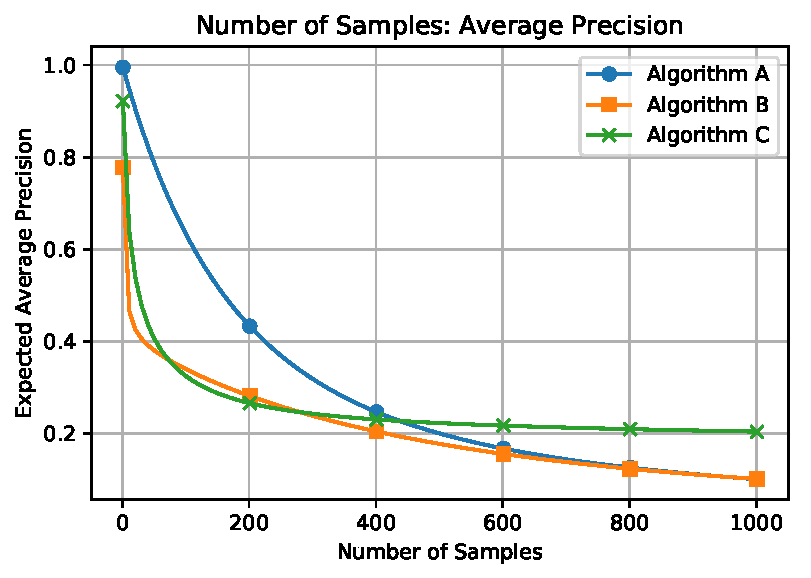
\includegraphics[width=0.49\textwidth]{figures/ex_num_samples_vs_ap.pdf}
    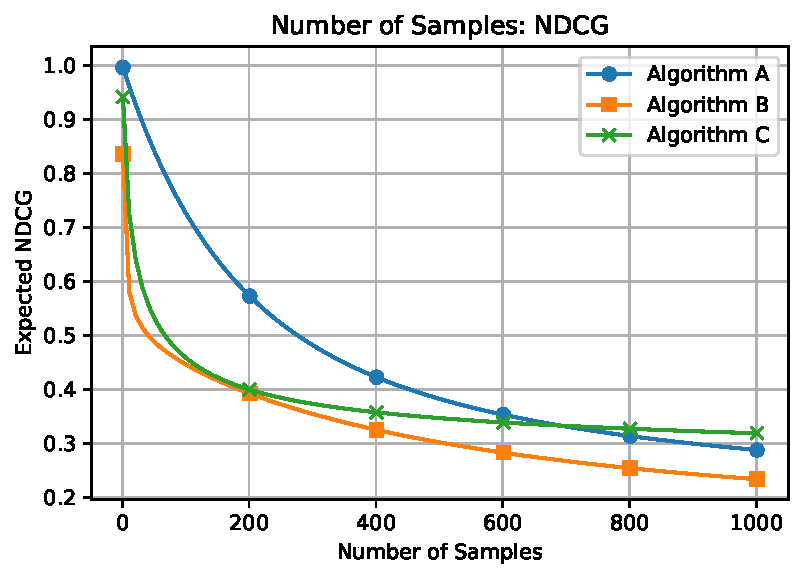
\includegraphics[width=0.49\textwidth]{figures/ex_num_samples_vs_ndcg.pdf} \newline
    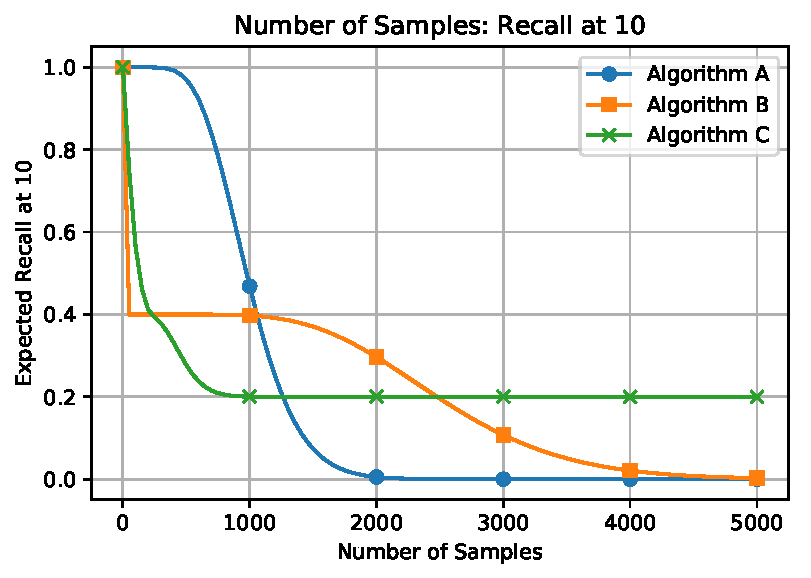
\includegraphics[width=0.49\textwidth]{figures/ex_num_samples_vs_recall.pdf}
    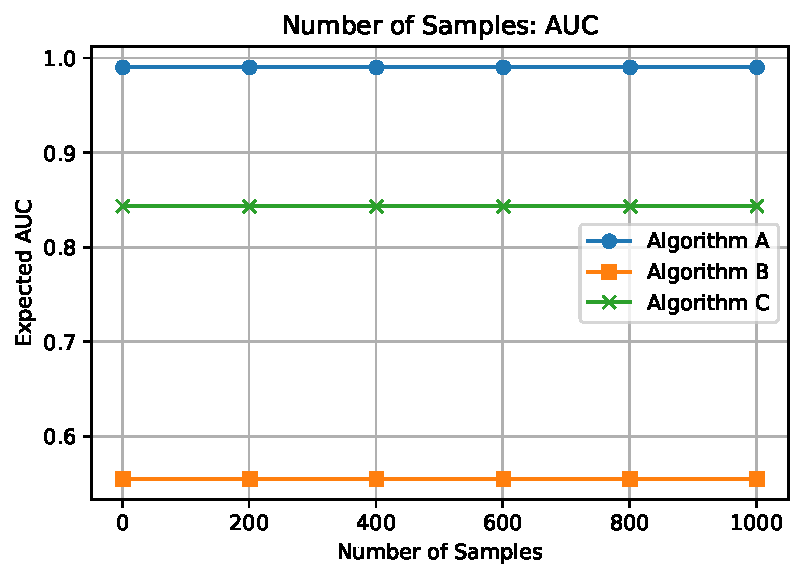
\includegraphics[width=0.49\textwidth]{figures/ex_num_samples_vs_auc.pdf}
    \caption{\footnotesize{Expected sampling metrics for the running example while increasing the number of samples.
    For Average Precision, NDCG and Recall, even the relative order of algorithm performance changes with the number of samples.
    That means, conclusions drawn from a subsample are not consistent with the true performance of the algorithm.}}
    \label{fig:example_vary_m}
\end{figure}

Из экспериментов видно, что единственная консистентная метрика --- \texttt{ROC AUC}.

\subsection*{Corrected Metrics}

Очень рекомендую самостоятельно ознакомиться с данной частью работы, так как ее не очень удобно излогать в виде конспекта.

\section*{Выводы}

\dbox{\textbf{Key Takeaways}:
\begin{enumerate}
    \item Нужно избегать сэмплирования при расчете метрик
    \item Если нет возможности избежать сэмплирования, то нужно использовать скорректированные версии метрик
    \item Вычисление метрик нужно повторять несколько раз с разным seed'ом для того чтобы уменьшить дисперсию
\end{enumerate}}

Все это в лишний раз наводит на мысли о том, что в ряде работ лучшими оказались алгоритмы, которые не обязательно являются лучшими на самом деле, и на результаты экспериментов в статьях всегда надо смотреть с определенной долей скепсиса.

\chapter{Temporal-Contextual Recommendation in Real-Time}

\textbf{Best ADS paper}

\textbf{Reference:}~\url{https://dl.acm.org/doi/pdf/10.1145/3394486.3403278}

\textbf{Keywords:} 

\section{Какую задачу решают авторы?}

\section{Как решают?}

\section{Преимущества подхода}


\section{Мое мнение}

% \chapter{Joint Optimization of Multiple Objectives on Music Streaming Platforms}
% \cite{rishabh2020multiobjective}

% \chapter{SimClusters: Community-Based Representations for Heterogeneous Recs at Twitter}
% \url{https://dl.acm.org/doi/pdf/10.1145/3394486.3403370}

% \chapter{Managing Diversity in Airbnb Search}
% \cite{abdool2020managing}

% \chapter{Multitask Mixture of Sequential Experts for User Activity Streams}

\chapter{Другие работы}

\section{Embedding-based Retrieval in Facebook Search}

Facebook \\

\textbf{Reference:}~\url{https://arxiv.org/abs/2006.11632}

\textbf{Конспект:}~\url{https://vk.com/@papersreaders-embedding-based-retrieval-in-facebook-search} \\

Исторически поиск в Facebook работал на основе Boolean matching model.

В статье авторы делятся опытом перехода к использованию embedding-based системы на этапе отбора кандидатов перед ранжированием. \\

В основе предлагаемого решения модель построения эмбеддингов запросов и документов. \\

Работа наглядно показывает, что даже относительно несложное решение для Embedding-based retrieval показывает существенное улучшение в сравнении с классическим Boolean matching подходом в задаче отбора кандидатов.

\section{Controllable Multi-Interest Framework for Recommendation}

Alibaba \\

\textbf{Reference:}~\url{https://arxiv.org/abs/2005.09347}

\textbf{Конспект:}~\url{https://vk.com/@papersreaders-controllable-multi-interest-framework-for-recommendation} \\

Современные рекомендательные системы используют историю пользователя для построения вектора, который описывает пользователя и используется для поиска объектов-кандидатов при построении рекомендаций. 

Однако использование единственного вектора для описания пользователя не позволяет уловить его разнообразные интересы. \\

Авторы статьи предлагают решение, которое позволяет представить пользователя в виде набора из К векторов, каждый из которых соответствует некоторому интересу пользователя.

Данный подход позволяет делать рекомендации как более точными так и более разнообразными в сравнении с существующими state-of-the-art подходами.

\section{PinnerSage: Multi-Modal User Embedding Framework \\ for Recommendations at Pinterest}

Pinterest \\

\textbf{Reference:}~\url{https://arxiv.org/pdf/2007.03634.pdf} \\

Статья от Pinterest про прокачку системы рекомендаций пинов для пользователя. \\

Авторы статьи рассматривают проблемы связанные с представлением пользователя в виде единственного вектора.

Для решения проблем, в статье предлагают представить пользователя в виде набора векторов. \\

Ключевые отличия от предыдущих работ, предлагающих сделать тоже самое:
\begin{enumerate}
    \item количество векторов для пользователя не фиксировано
    \item вектора для пользователей не обучаются совместно с векторами для пинов
\end{enumerate}

Для того чтобы представить пользователя в виде набора векторов, предлагают делать иерархическую кластеризацию активности пользователя за последнее время (вектора пинов получены black-box моделью).

Каждому кластеру ставят в соответствие его важность.  \\

Для рекомендации релевантных пинов берут 3 наиболее важных кластера и ищут похожие пины с помощью приближенного поиска ближ соседей. \\

Как и в большинстве последних статей от Pinterest, авторы рассматривают продакшн решение, поэтому достаточно внимания уделяют вопросу о том как все это тащить в прод.

\section{Improving Recommendation Quality in Google Drive}

Google \\

\textbf{Reference:}~\url{https://research.google/pubs/pub49272/} \\

Статья про попытки прокачать качество инструмента Quick Access (статья не научная, а просто про опыт и проведенные эксперименты) \\

В целом, то о чем они пишут очень похоже на наш опыт и на наши эксперименты за последние года полтора. \\

Эксперименты описанные в статье, которые похожие на наши
\begin{itemize}
    \item автоматизация пайплайнов переобучения моделей
    \item попытки затащить DL модели (в статье наоборот пытаются перейти к GBDT)
    \item изучение того как влияет latency на метрики
    \item несколько примеров feature engineering'a 
    \item эксперимент с увеличением числа кандидатов для ранжирования
    \item фича мониторинг
\end{itemize}

\addcontentsline{toc}{chapter}{Литература}
\putbib[refs_recsys]
\end{bibunit}
